\chapter{DIMENSIONAMIENTO DEL EJE Y TRANSMISIÓN PARA EL ACCIONAMIENTO DISTANTE DEL POLIPASTO E IZAJE DE LA CARGA A LA MITAD DEL TIRANTE O TRAVESAÑO DE APOYO. }
\begin{center}
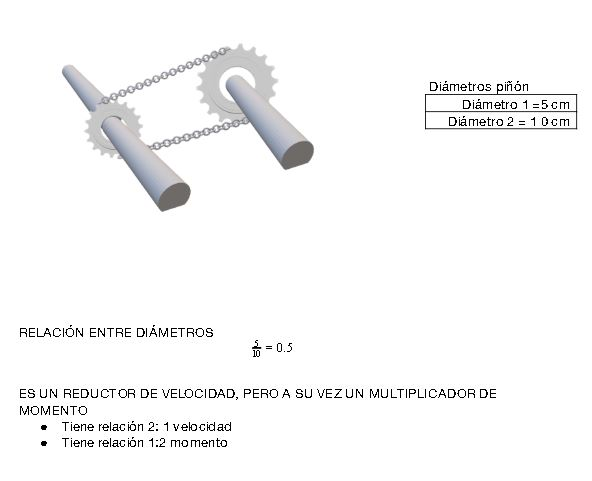
\includegraphics[width=0.9\linewidth]{D/figs/DI_1.jpg} 
\end{center}

\begin{center}
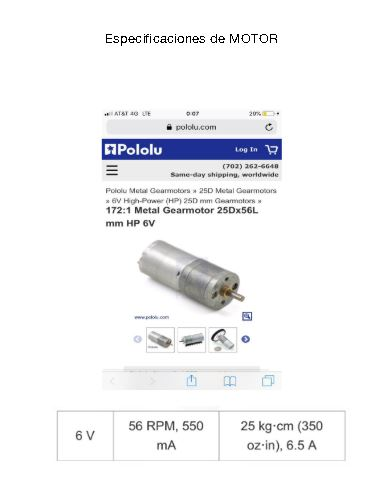
\includegraphics[width=0.7\linewidth]{D/figs/DI_2.jpg} 
\end{center}

\begin{center}
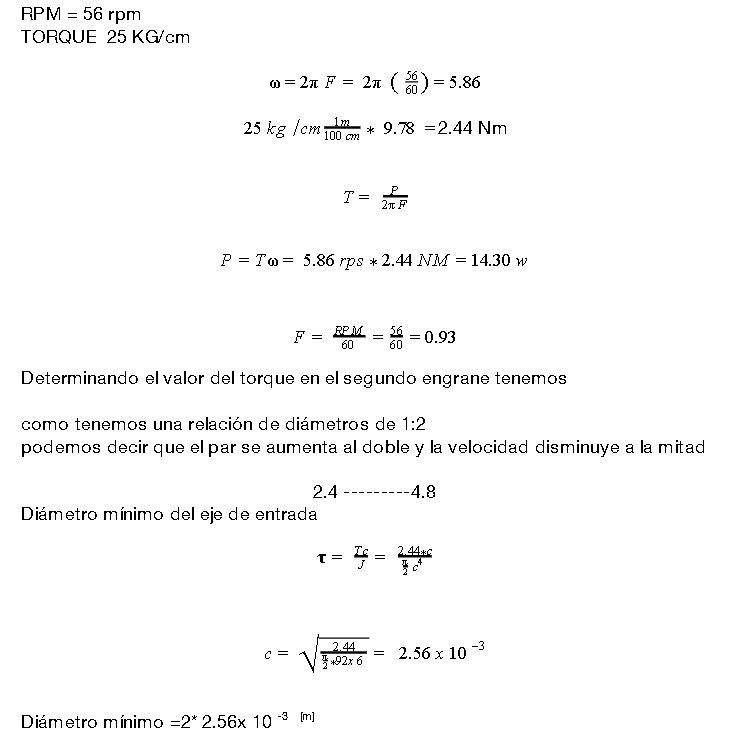
\includegraphics[width=0.9\linewidth]{D/figs/DI_3.jpg} 
\end{center}

\section{Selección del material}

\makebox[\textwidth]{Aluminio} \par
Escogimos aluminio para el eje debido a que tiene las propiedades mecánicas que cumplen con nuestros requisitos. 
\\
\begin{table}[htb]
\centering

\begin{tabular}{| p{2.8cm}| p{2.8cm} | p{2.8cm} |}
\hline
\multicolumn{3}{|c|}{Aluminio} \\
\hline
$\tau$ & E &  G  \\
\hline \hline \hline
92 MPa & 70.6 GPa  & 26.3 GPa \\ \hline
\end{tabular}
\caption{Propiedades mecánicas}
\label{}
\end{table}

\textrm{Se utilizó el $\tau$y= 92 MPa debido a que el valor de esfuerzo de $\sigma$y= 125 MPa}

\textrm{Lo anterior se basa en el siguiente criterio: } \href{http://minisconlatex.blogspot.com/2012/03/guiones-y-comillas.html}{ ``La resistencia a cizallamiento es un valor importante a tener en cuenta para calcular la fuerza necesaria para el corte, así como para determinadas construcciones. No existen valores normalizados a este respecto, pero generalmente es un valor que está entre el 55 y 80 porciento de la resistencia a la tracción.''}

\bigskip
\bigskip
\bigskip
\bigskip
\textrm{Módulo de elasticidad longitudinal o Módulo de Young}

\begin{center}
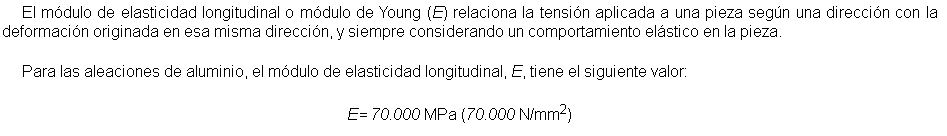
\includegraphics[width=0.9\linewidth]{D/figs/D_3.jpg} 
\end{center}


\textrm{de acuerdo con el proveedor del material tenemos}
\begin{center}
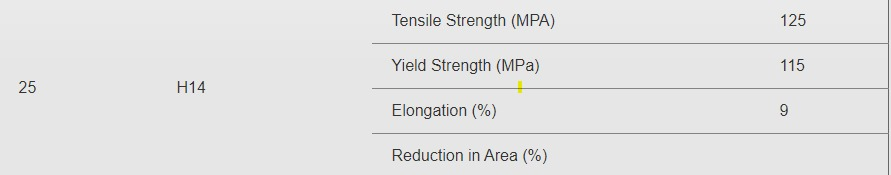
\includegraphics[width=0.9\linewidth]{D/figs/D_4.jpeg} 
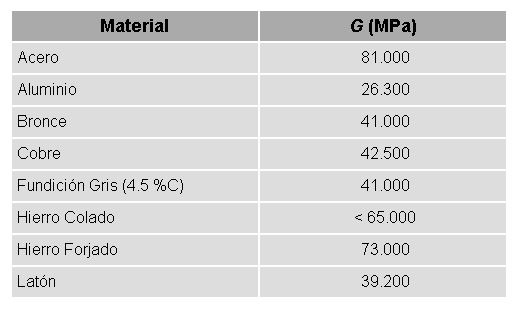
\includegraphics[width=0.9\linewidth]{D/figs/D_5.jpg} 
\end{center}

\section{Esfuerzo y Deformación máxima, (DMF y DEC).}

\begin{table}[htb]
\centering
\begin{tabular}{| p{2.2cm}| p{2.2cm} |}
\hline
\multicolumn{2}{|c|}{Aluminio} \\
\hline
E & G \\
\hline \hline
70 GPa & 26.3 GPa  \\ \hline
\end{tabular}
\caption{Propiedades mecánicas}
\label{}
\end{table}


\section{Determinación de diámetro.}

\begin{center}
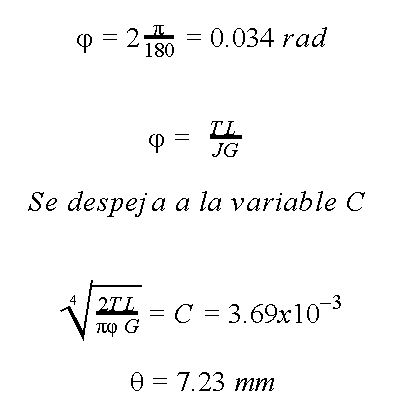
\includegraphics[width=0.6\linewidth]{D/figs/DB_1.jpg} 
\end{center}

\begin{equation*}
\textrm{ Diámetro } = 8 \textrm{ mm }
\end{equation*}
\begin{equation*}
\textrm{ Longitud } = 10 \textrm{ cm}
\end{equation*}
\begin{equation*}
\textrm{ Radio } = 4 \textrm{ mm }
\end{equation*}

\begin{equation} 
\begin{split}
\tau & = \frac{T C}{J} \\
\end{split}
\end{equation}


\begin{center}
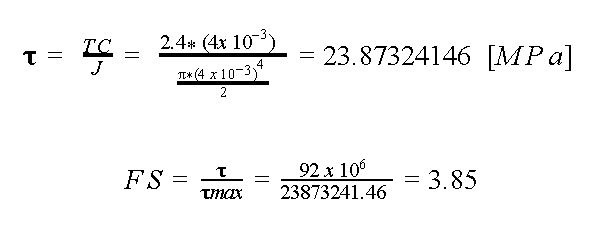
\includegraphics[width=0.6\linewidth]{D/figs/DB_2.jpg} 
\end{center}


\section{Deformaciones en el eje.}

\begin{equation} 
\begin{split}
J & = \frac{\pi C^2}{2} \\
  & = \frac{\pi (8x10^{-3})^2}{2} \\
  & = 1.0052x10^{-4} [m^{4}]\\
\gamma & = \frac{2.4516625*8x10^{-3}}{1.0052x10^{-4}*26.3x10^{9}} \\
       & = 7.4181x10^{-9} [rad]\\
       & = 4.25x10^{-9} [grados]
\end{split}
\end{equation}